\documentclass[a4paper,11pt]{article}

%Les packages pour écrire des math
\usepackage{amsmath}
\usepackage{amsthm}
\usepackage{amssymb}
\usepackage{mathabx}
\usepackage{dsfont} %Fonction caractéristique
\usepackage{stmaryrd}
\numberwithin{equation}{section}

\usepackage{listings}
\usepackage[authoryear]{natbib}


\usepackage{hyperref}
\usepackage{url}

\usepackage{algorithm}
\usepackage{algorithmic}

%\usepackage[francais]{babel}	
\usepackage[utf8]{inputenc}
%\usepackage[T1]{fontenc}

\usepackage{graphicx}
%\usepackage{pst-solides3d}
\graphicspath{ {./images/} }
\usepackage[font=small,labelfont=bf]{caption}
\usepackage{subcaption}


\textwidth16cm
\oddsidemargin-0.55cm
\textheight21.5cm
\topmargin-1cm
\pagestyle{plain}
\setlength{\skip\footins}{1.2cm}


\renewcommand {\algorithmicrequire } {\textbf{\textsc{Entrée(s):} } }
\renewcommand {\algorithmicensure } {\textbf{\textsc{Sortie:} } }
\renewcommand {\algorithmicwhile } {\textbf{Tant que} }
\renewcommand {\algorithmicdo } {\textbf{faire} }
\renewcommand {\algorithmicendwhile } {\textbf{fin du Tant que} }
\renewcommand {\algorithmicif } {\textbf{Si} }
\renewcommand {\algorithmicfor } {\textbf{Pour} }
\renewcommand {\algorithmicendfor } {\textbf{fin du Pour} }
\renewcommand {\algorithmicthen } {\textbf{alors} }
\renewcommand {\algorithmicendif } {\textbf{fin du Si} }
\renewcommand {\algorithmicelse } {\textbf{Sinon} }
\renewcommand {\algorithmicreturn } {\textbf{Renvoyer} }

\newtheorem{theorem}{Théorème}[section]
\newtheorem{conjecture}{Conjecture}
\newtheorem{lemma}{Lemme}
\newtheorem{proposition}{Proposition}
\newtheorem{corollary}{Corollaire}
\newtheorem{definition}{Définition}
\newtheorem{example}{Exemple}
\newtheorem{note}{Note}



\begin{document}
	\begin{center}
			
\includegraphics[scale=0.5]{images/LSCE.jpg}
	\end{center}
	\hypersetup{pdfborder=0 0 0}
	\newcommand{\HRule}{\rule{\linewidth}{0.5mm}}
	\begin{center}
		\textsc{\LARGE Laboratoire des Sciences du Climat} \\[0.3cm]
		\textsc{\LARGE et de l'Environnement}\\[1.5cm] 
		\HRule \\[0.5cm]
		{\huge \bfseries Changement d’échelles dans les projections climatiques et leurs impacts hydrologiques: Cas des grandes plaines américaines}\\[0.4cm] 
		\HRule \\[1.5cm]
	\end{center}
	\begin{minipage}{0.4\textwidth}
		\begin{flushleft} \Large
			\emph{Auteur}\\
		\end{flushleft}
	\end{minipage}
	~
	\begin{minipage}{0.4\textwidth}
		\begin{flushright} \Large
			\emph{Maîtres de stage} \\
		\end{flushright}
	\end{minipage}\\[0.5 cm]
	\begin{minipage}{0.4\textwidth}
		\begin{flushleft} \large
			\textsc{Mathis Deronzier}\\
			\textsc{Mines Saint-Étienne}
		\end{flushleft}
	\end{minipage}
	~
	\begin{minipage}{0.4\textwidth}
		\begin{flushright} \large
			\textsc{Emmanuel Mouche}\\
			\textsc{C.E.A.}\\
			\textsc{Mathieu Vrac}\\
			\textsc{C.N.R.S.}
		\end{flushright}
	\end{minipage}\\[2cm]
	\begin{center}
		\textsc{\Large Stage de recherche de master 2}\\[0.5cm]  
		\large Avril-Septembre\\2021\\[2cm]
	\end{center}

\newpage
\tableofcontents

\newpage
\section{Introduction}
\label{ch:introduction}

\subsection{Contextualisation et motivations du stage}
\label{ch:Contextualisation et motivations du stage}

Alors que le rapport du GIEC 2021 sorti cet été projette une augmentation de la température mondiale moyenne de $1.5^{\circ}$C d'ici $2050$ ainsi que des modifications des climats dans plusieurs régions du monde. Il semble aujourd'hui primordial de comprendre les conséquences locales d'un changement climatique global. Les changements climatiques locaux sont des enjeux politiques et économiques majeurs et leurs prévisions sont des problématiques centrales pour la population mondiale.

Les projections climatiques sont données par des modèles de climat travaillant à l'échelle de l'ordre d'une centaine de kilomètres, on cherche alors à prévoir des résultat sur des zones plus localisées. Le domaine du climat étudiant les questions de changement d'échelle du global au local est le \textit{downscaling}. La question inverse du changement d'échelle du local au global est non moins intéressante pour les climatologues. En effet, comment savoir si les modèles à grande échelle sont vraiment représentatifs de la réalité? Alors que les modèles climatiques et hydrologiques travaillent sur des échelles globales, les lois de la physique sont elles, locales. On cherche alors à comprendre à partir des équations de la physique les interactions ou équations qu'elles engendrent à grande échelle, ce domaine de recherche s'appelle l'\textit{upscaling}. 

C'est dans ces problématiques de changement d'échelles que s'ancre ce stage. Pour concentrer et enrichir nos réflexions, nous nous intéresserons plus précisément à la question de l'impact du changement d'échelle sur les modélisations hydrologiques. Afin de concrétiser ces problématiques, nous avons modélisé le fonctionnement hydrologique du bassin du Little Washita. 
Le domaine d'étude ayant été choisi pour modéliser et concrétiser ces problématiques a été le bassin du Little Washita. Ce bassin situé aux États-Unis dans l’état d’Oklahoma, possède de nombreuses caractéristiques qui le rendent intéressant. Sa superficie de $611km^2$ est de l'ordre de grandeur d'une maille de modèle continentale et il a déjà fait l'objet de nombreuses études (voir par exemple \cite{maxwell2007groundwater}, \cite{rosero2011ensemble}, \cite{maquin2016developpement}). 

\vspace{0.7cm}

Pour s'intéresser à la question du changement d'échelle il fallait pouvoir comparer des données à grande échelle et à petite échelle. Les données NARR (North American Regional Reanalysis\footnote{Les reanalysis sont des modèles de climats simulés que l'on force à prendre certaine valeurs mesurées pour certains points et certains temps, nous considérerons les données NARR comme les données climatiques réelles.}) allant de l'année $1979$ à $2014$ semblaient constituer un jeux de données pertinent pour l'étude du Little Washita. En effet, sa longueur de maille de $32km$ permettait à la fois de considérer l'upscaling hydrologique sur de ce bassin et le downscaling pour des jeux de données sur des échelles plus larges. Pour obtenir ces données à grande échelle nous avons opté pour deux types de données: les données l'IPSL qui possède une longueur de maille de $200km$ ainsi que des données obtenues en faisant des dégradations spatiales sur les données NARR. Ainsi, si les données IPSL et NARR sont peut-être décorrélées on est absolument certain que les données NARR et leurs dégradées le sont. L'objectif aura été dans un premier temps de regarder différentes méthodes de downscaling pour améliorer les projections des données NARR à partir des séries à plus grande échelle. Une fois effectuée cette étape il s'agissait de réaliser une simulation hydraulique sur les années prédites et de comparer l'impact du downscaling sur les résultats des simulations hydrologiques. La problématique de l'upscaling sera en fait cachée dans la modélisation hydrologique du bassin du Little Washita, bien qu'elle n'ait pas été concrètement traitée dans les faits, elle a été centrale dans notre réflexion. Finalement nous avons donné les conclusions que nous avons tirées dans.

\subsection{Présentation du plan}
\label{ch:presentation plan}

Dans la première partie nous allons introduire rigoureusement le concept de downscaling et les outils utilisés pour mesurer la qualité de nos prédictions. Nous verrons l'algorithme \textit{Cumulative Distribution Function transfert} (CDF-t), celui utilisé pour downscaler nos séries. Nous introduirons le transport optimal généralisant l'algorithme CDF-t. Nous verrons ensuite comment estimer la qualité de nos prédictions, alors on étudiera les distances de Kolmogorov Smirnov et celle de Cramér-von Mises permettant de quantifier la différence entre deux lois. 

La seconde partie sera consacrée à la physique et la modélisation, elle présentera les principaux mécanismes de la modélisation hydrologique ainsi que les modèles d'Orchidée et d'HydroGéoSphère. Dans un premier temps nous présenterons les interactions sol-atmosphère ainsi que les caractéristique des sol et leur influence sur les débits. Nous présenterons ensuite les principales équations de la mécanique des fluides en milieu poreux, puis deux modèles utilisés pour les modélisations hydrologiques, Orchidée et HydroGéoSphère en expliquant plus en détail la problématique de l'upscaling.

La troisième et dernière partie présentera la démarche les résultats ainsi que les questionnements que nous avons eu au cours de ce stage. Nous commencerons par expliquer en détail la méthodologie que avons suivi, puis nous présenterons pas à pas les résultats que nous avons obtenus.



\newpage
\section{Changement d'échelle, downscaling et analyse des résultats}
\label{ch:downscaling}
Cette section se concentre sur la partie statistique du stage, on cherchera à partir de données à grande échelle issues de modèles climatiques et de données réelles à améliorer les projections de la précipitation et de l'évapotranspiration sur le bassin versant du Little Washita. 

\vspace{0.7cm}

Nous commencerons par formaliser rigoureusement le downscaling statistique, puis nous réintroduirons les concepts mathématiques essentiels à la compréhension de l'algorithme CDF-t. Nous verrons ensuite comment on peut généraliser le principe de l'algorithme CDF-t avec la méthode du transport optimal. Pour terminer nous verrons les méthodes de test pour évaluer la qualité de prédictions sur plusieurs année

\vspace{0.7cm}

Le downscaling statistique (voir par exemple \cite{vrac2012dynamical} et \cite{ayar2016intercomparison}) est une méthode utilisée dans les sciences du climat permettant d'améliorer les projections des modèles climatiques. À partir des données obtenues par un modèle climatique (modèle de circulation général, modèle climatique régional) et des données observées, on cherche à observer et corriger les biais systématiques introduits par les modèles. Le nom ``downscaling'' vient du domaine d'application de cette méthode. On passe d'un modèle à grande échelle à des données observées à petite échelle. Cette méthode est très utile dans la pratique où l'on a des modèles de climat donnant des résultats sur des maillages de grande échelle ($\sim 200km\times 200km$). Dans notre cas, nous utilisons le downscaling pour projeter les variables climatiques de \textit{précipitation} et d'\textit{évapotranspiration} sur le bassin du Little Washita. Nous n'expliquerons que deux méthodes de downscaling mais d'autres méthodes existent, l'article de \cite{ayar2016intercomparison} donne un aperçu des différentes méthodes.
Nous n'avons testé qu'une méthode de downscaling mais d'autre existent. Nous l'avons testée à partir du jeux de données: les données NARRs (de taille de grille de $30km\times 30 km$) ainsi que celles de l'IPSL (de taille de grille de $200km\times200 km$), nous détaillerons ce travail dans la section \ref{ch: pred-cli}.

\vspace{0.7cm}

Pour formuler rigoureusement l'approche du downscaling nous introduisons des hypothèses communément admises dans les sciences du climat. On suppose que les variables étudiées sont des variables aléatoires réelles dépendantes du temps et de l'espace, on appelle $\mathcal{M}(\Omega,\mathbb{R})$ l'espace des variables aléatoires réelles et $S(\mathbb{R}^3)$ la spère unité dans $\mathbb{R}^3$. On suppose de plus que l'on peut faire correspondre chaque point de la terre à un point de la sphère unité. Nous travaillerons par la suite sur la sphère unité que l'on considérera être la terre.

\begin{definition}
	\label{terre}
	Pour une variable quantitative $V$ à valeur dans $\mathbb{R}$, on appelle $\mathcal{T}_V$ la fonction donnant les  valeurs réelles de cette variable sur la terre à un moment donné, formellement (en considérant la terre comme une sphère $\mathcal{S}(\mathbb{R}^3)$) nous avons
	\begin{equation}
		\begin{array}{ccc}
			\mathcal{T}_V: \mathbb{R}_{+}\times\mathcal{S}(\mathbb{R}^{3}) & \to & \mathcal{M}(\Omega,\mathbb{R}).
		\end{array}
	\end{equation}
	Alors, $\mathcal{T}_V(t,x)$ est la valeur de la variable au temps $t$ au point de coordonnée $x$ sur terre.	
\end{definition}

\begin{definition}
	\label{simu_terre}
	On appelle simulateur de variable quantitative $V$ à valeur dans $\mathbb{R}$, une fonction $S_V$ satisfaisant:
	\begin{equation}
		\begin{array}{ccc}
			S_V: \mathbb{R}_{+}\times\mathcal{S}(\mathbb{R}^{3}) & \to & \mathcal{M}(\Omega,\mathbb{R}).
		\end{array}
	\end{equation}
\end{definition}
On peut alors estimer la qualité des simulations en mesurant une distance entre la réalisation $\mathcal{T}_V([0,T])$ et celle de $S_V([0,T])$. Le travail du downscaling est de trouver des transformations sur les variables aléatoires $S_V(t,x)$ pour minimiser ces distances. Plusieurs méthodes peuvent-être utilisées pour réduire ces distances. Les géostatistiques essaient entre autres d'étudier la structure de covariance sur l'espace sur lequel on considère ces variables. Des méthodes de résolution d'équations différentielles permettent d'interpoler les résultats (voir par exemple \cite{lindgren2011explicit}). Nous ne donnons qu'un bref apercu de ces méthodes puisque ce ne sont pas celles-ci que nous allons étudier.

\subsection{Introduction à la problématique du downscaling}
\label{ch:intro-dwnsc}
Le downscaling consiste donc à effectuer des transformations sur des variables aléatoires réelles. Pour étudier ces variables aléatoires et construire les transformation on commence par introduire ici les notions de \textbf{fonction de répartition}, \textbf{fonction de répartition empirique} ainsi que celle de \textbf{fonction de densité}. Ces notions sont centrales dans les méthodes de downscaling que nous allons expliquer.

\begin{definition}
	Soit $X$ une variable aléatoire réelle, on appelle \textbf{fonction de répartition de $X$}, $\mathcal{F}_{X}: \mathbb{R}\to [0,1]$ la fonction vérifiant
	\begin{equation}
		\mathcal{F}_{X}(x)=P(X\leq x).
	\end{equation}
\end{definition}

\begin{definition}
	Soient $X_1,X_2,...,X_n$, n réalisations indépendantes d'une variable aléatoire réelle $X$, on appelle \textbf{fonction de répartition empirique de $X$}, la fonction $\mathcal{F}_{n}:\mathbb{R}\to [0,1]$ définie par
	\begin{equation}
		\mathcal{F}_{n}(x)= \frac{1}{n}\sum_{i=1}^{n}\mathds{1}_{[X_i, +\infty )}(x).
	\end{equation}
\end{definition}

\begin{definition}
	Soit $X$une variable aléatoire réelle, on note $f_{X}$ la \textbf{fonction de densité de $X$}, $f_{X}: \mathbb{R}\to [0,\infty[$ la fonction vérifiant
	\begin{equation}
		f_{X}(x)=\lim_{t\to 0} \frac{P(x\leq X \leq x+t)}{t}.
	\end{equation}
\end{definition}
Remarquons qu'une variable aléatoire ne possède pas nécessairement de fonction de répartition (notamment les variables aléatoires à valeurs discrètes), on peut cependant les étudier dans la théorie des distributions \cite{golse2020distributions}.

Commençons par établir notre problématique dans le cas le plus simple où l'on cherche à projeter une variable $V$ dans l'avenir alors que nous connaissons ses réalisations dans le passé à un endroit donné $x$.
On peut alors considérer deux processus aléatoires à valeurs dans $\mathbb{R}$, 
\[(X_t)_{t \in \mathbb{N}}=(\mathcal{S}_{V}(t, x))_{t \in \mathbb{N}} \textrm{ et } (Y_t)_{t \in \mathbb{N}}=(\mathcal{T}_{V}(t, x))_{t \in \mathbb{N}}.\]

La problématique à laquelle nous cherchons de répondre est la suivante: connaissant $X_1,X_2,...,X_n$ et $Y_1,Y_2,...,Y_n$ les réalisations jusqu'au temps $n$ ainsi que $X_{i_1},X_{i_2},...,X_{i_m}$ (pour des temps futurs), on cherche une fonction $G: \mathbb{R} \to \mathbb{R}$ telle que les tirages $G(X_{i_1}),..., G(X_{i_m})$ et $Y_{i_1},...,Y_{i_m}$ soient proches du point de vu de leur loi (nous éclaircirons ce point par la suite dans la section \ref{analyse-pred}). 

Autrement dit, en appelant $X$ et $Y$ les réalisations de $(X_t)_{t \in \mathbb{N}}$ et $(Y_t)_{t \in \mathbb{N}}$ sur $\{1,...,n\}$ et $X'$ et $Y'$ les réalisations de $(X_t)_{t \in \mathbb{N}}$ et de $(Y_t)_{t \in \mathbb{N}}$ sur $\{i_1,...,i_m\}$, on cherche à définir $G_{X,Y}$ à partir de $X$, $Y$ tel que $G_{X,Y}$ minimise 
\[d(\mathcal{F}_{G_{X,Y}(X')}, \mathcal{F}_{Y'}),\]
où $d$ est une distance définie sur les fonctions.
Nous voulons aussi que $G_{X,Y}$ respecte certaines propriétés. Une des propriété qui nous intéresse est celle de la consistance de notre transformation.

\begin{definition}
	Soient $X$ et $Y$ deux variables aléatoires réelles et $G_{X,Y}: \mathbb{R}\to \mathbb{R}$ une transformation, on dit que $G_{X,Y}$ est \textbf{consistante vis à vis de $X$ et de $Y$} si elle vérifie 
	\begin{equation}
		\label{cond-cons}
		{\mathcal{F}_{G_{X,Y}(X)}}= \mathcal{F}_{Y}.
	\end{equation}
\end{definition}
Dans la suite les transformations que nous considérerons satisferont toujours l'équation \eqref{cond-cons}.

\subsection{Cumulative Distribution Function transform (CDFt)}
\label{ch:CDFt}

Nous allons ici présenter l'algorithme principalement étudié et utilisé dans ce stage, l'algorithme CDF-t (voir \cite{vrac2012dynamical}). Nous commencerons par présenter l'algorithme quantile-quantile (voir ) permettant de comprendre l'esprit des transformations $G$ affectées aux processus aléatoires. Puis nous décrirons l'algorithme de CDFt-t. 

\subsubsection{Quantile-Quantile}
\label{Q-Q}
Le quantile-quantile consiste simplement à définir $G_{X,Y}$ la transformation permettant de passer de la fonction de distribution de $X$ à celle de $Y$. 
\begin{proposition}
	\label{prop:QQ_formula}
	Soit $X$ et $Y$ deux variables aléatoires réelles ayant des fonctions de répartition $\mathcal{F}_{X}$ et $\mathcal{F}_{Y}$ continues, alors 
	$\mathcal{F}^{-1}_Y (\mathcal{F}_X(X))$ et $Y$ suivent la même loi. 
\end{proposition}
On peut retrouver la démonstration de cette proposition dans les annexes section \ref{ch:outils-mathematiques}. Le principe de l'algorithme \textbf{quantile-quantile} est alors de calculer la transformation $G=\mathcal{F}^{-1}_{Y} \circ \mathcal{F}_{X}$. Ainsi, $\mathcal{F}_{G(X)}=\mathcal{F}_{Y}$ et l'on définit alors $G_{X,Y}=G$. L'une des limites de cette méthode est que le support de $f_{G(X)}$ est inclus dans celui de $f_{Y}$, alors les valeurs prises par $G_{X,Y}(X')$ seront incluses dans le support de $f_Y$. Nous aimerions que $X'$ ait aussi une influence sur le support des valeurs prises. Ce qui n'est pas le cas dans la transformation $G$ défini par la proposition \ref{prop:QQ_formula}. C'est en partie cette observation qui motive l'étude d'autres transformations. 

\subsubsection{CDFt}
\label{CDf-t-algo}

L'algorithme de \textbf{Cumulative Distribution Function transfer} (CDFt) vise à remédier au problème des bornes en appliquant des transformations sur les lois $X$ et $Y$. On considère les réalisations $X_1,..,X_n$ et $Y_1,...,Y_n$ ainsi que $X'_{1},...,X'{m}$.

\noindent \textbf{CDFt avec support égale}:

On peut par exemple faire en sorte que la transformation sur les projections conserve le support de celles-ci en d'autres mots on veut
\[ \min_{i \in I}(X'_i)=\min_{i \in I}(G_{X,Y}(X'_i)) \hspace{3mm} \textrm{et} \hspace{3mm}  \max_{i \in I}(X'_i)=\max_{i \in I}(G_{X,Y}(X'_i)).\]
Il suffit de transformer la loi de $Y$ sur $[0,1]$, de réaliser un quantile-quantile puis d'effectuer la transformation inverse. Concrêtement, nous posons 
\[\overset{\sim}{Y}= \frac{(Y-\min_{i\in I}Y_i)}{\max_{i\in I}Y_i- \min_{i\in I}Y_i}.\]
Alors quelque soit $i$ dans $\mathcal{I}$ on a $\overset{\sim}{Y}_i \in [0,1]$. En appelant $G= \mathcal{F}_{X,\overset{\sim}{Y}}$ la transformation quantile-quantile de $X$ à $\overset{\sim}{Y}$ on a $G_{X,Y}(X'_i) \in [0,1]$, la transformation s'imposant naturellement est alors
\[ G_{X,Y}= (\max_{i\in I}Y_i- \min_{i\in I}Y_i)G + \min_{i\in I}Y_i.\]
C'est l'une des premières idées qui vienne-t-en tête lorsqu'on parle de transformations que l'on peut appliquer sur nos variables. Notons que l'on a aussi une grosse base de données et que l'on peut aussi essayer d'utiliser des méthodes de regression linéaire ou de machine learning pour estimer les max et les min de $Y'$ en fonction de $X$. Nous allons illustrer l'usage d'une de ces méthodes dans la prochaine partie \ref{CDFt reg l}.

\noindent \textbf{CDFt avec méthode de prédiction}
\label{CDFt reg l}

Supposons que l'on ait des fonctions estimant la variance et la moyenne de $Y'$ à partir de $X'$, s'exprimant sous la forme $\overline{f(X')} = \overline{Y'}$ ainsi que $\overline{g(X')} = \overline{\sigma(Y')}$ \footnote{On définit par $\overline{X}$ la  moyenne $X$ et par $\sigma(X)$ son écart type.}. Ces fonctions peuvent être obenues par des méthodes de régression linéaire sur des sous échantillons des données de $X$ et $Y$ soit après les avoir ordonnées si les $X_i$ et les $Y_i$ sont indépendants soit en fonction de leur indice.

On aimerait alors que $G_{X,Y}$ conserve la moyenne ainsi que la variance. Formellement, on voudrait définir $G_{X,Y}$ telle que quelque soient $\{i_1,...,i_m\}$ un ensemble d'entiers consécutifs et $X'$ et $Y'$ les vecteurs des variables aléatoires des $X_{i_j}$ et $Y_{i_j}$ sur cet ensembles, on ait :

\begin{equation}
	\label{cond-mu}
	\overline{G_{X,Y}(X')}=\overline{Y'},
\end{equation}
ainsi que
\begin{equation}
	\label{cond-sigma}
	\sigma({G_{X,Y}(X')})=\sigma(Y'),
\end{equation}
et que $G$ respecte la condition de consistance \eqref{cond-cons}.
Concrêtement, nous allons faire des transformations sur les variables aléatoires pour avoir ces conditions là. En appelant $G_{X,Y}= \mathcal{F}^{-1}_{Y}\circ\mathcal{F}_{X}$ on peut définir la transformation $G_{X,Y,X'}$

\[ G_{X,Y} (X')= \overline{g(X')}\frac{\mathcal{F}^{-1}_{Y}\circ\mathcal{F}_{X}(X')- \overline{\mathcal{F}^{-1}_{Y}\circ\mathcal{F}_{X}(X')}}{\sigma(\mathcal{F}^{-1}_{Y}\circ\mathcal{F}_{X}(X'))} + \overline{f(X')}.\]

On peut vérifier facilement que $G_{X,Y}$ ainsi défini respecte bien les propriétés \eqref{cond-cons} \eqref{cond-mu} et \eqref{cond-sigma}. L'idée est alors de trouver les fonctions $f$ et $g$ par des méthodes de regression linéaires. Remarquons aussi que lorsque la loi est bornée cela ajoute une condition supplémentaire à $G_{X,Y}$ et l'on ne peut pas nécessairement avoir les conditions sur la moyenne et la variance. Il faut alors choisir parmi l'une des conditions \eqref{cond-mu} et \eqref{cond-sigma}, c'est par exemple le cas pour les précipitations qui ne peuvent être négatives. 
\begin{note}
	Remarquons que l'efficacité des transformations que nous avons décrites repose en partie sur la stationnarité des lois suivies par les variables aléatoires aléatoires au cours du temps. Les questions de stationnarité ont été abordées dans \cite{maraun2012nonstationarities}, \cite{christensen2008need} ainsi que \cite{nahar2017assessing}.  
\end{note}

Finalement, une des limites de l'algorithme de CDF-t est dans le cas où plusieurs valeurs de $X'$ sont égales elle seront envoyées sur le même points. C'est vraiment problématique dans le cas où $X'$ possède plusieurs réalisations égales et que $\mathcal{F}_Y$ est une fonction continue (sans Dirac).

\begin{example}
	Soit $X$ une variable aléatoire qui possède comme probabilité 
	\[P(X=0)=\frac{1}{2} \textrm{ et } P( \frac{1}{2}\leq a\leq X \leq b\leq 1 )=b-a.\]
	et $Y$ une variable aléatoire réelle suivant la loi uniforme sur $[0,1]$. Intuitivement, on aimerait que pour chaque $i\in \{1,...,n\}$ tel que $X_i=0$ $G(X_i)$ suivent une loi uniforme sur $[0,1/2]$ ce qui n'est pas possible avec les transformations que nous avons considérées.
\end{example}  

C'est en partie à ce problème que répond le transport optimal.

\subsection{Transport optimal}
\label{ch:transport-optimal}

Nous voulons à la fois projeter la précipitation et l'évapotranspiration, on peut alors considérer une seule variable aléatoire dans $\mathbb{R}^2$. On peut généraliser l'idée utilisée précédemment pour trouver une méthode permettant de corriger les biais statistiques introduits par les modèles de projection. Cette méthode a d'autant plus d'intérêt que la variable utile dans les modèles hydrologique est 
\begin{equation}
	\label{eq:Qin-pr-etp}
	\textit{quantité d'eau entrant dans le sol}=\textit{précipitation}-\textit{évapotranspiration}.
\end{equation}
Comme l'objectif final est de projeter des résultats hydrologiques sur le bassin du Little Washita, il semble particulièrement pertinent de considérer la loi conjointe (précipitation, évapotranspiration\footnote{Nous utiliserons en réalité l'évaporation potentielle et nous verrons dans la section \ref{ch:generalite interaction atmosphere-surface continentale-sol} qu'il faut encore travailler pour obtenir l'évaporation finale.}). La théorie généralisant cette idée est la théorie du \textbf{transport optimal}.

La problématique du transport optimal a premièrement été introduite en par Gaspard Monge en 1781 puis a été développée par Kantorovitch en $1971$ et ses travaux pour l'allocution des ressources lui ont valu un prix nobel d'économie en $1975$.

\subsubsection{Problématique}
\label{ch:s-Problematique}

Précédemment nous avons cherché à définir une transformation $G$ de la variable aléatoire $X$ telle $G(X)$ suive la même loi que $Y$. En considérant les fonctions de densité de $X$ et de $Y$ on a cherché à ce que la fonction de densité de $G(X)$ soit la même que celle de $Y$. On peut considérer une fonction de densité comme une mesure sur l'espace sur lequel on travail on a alors transformé une mesure $f_X$ en une autre mesure $f_Y$. Comme ces deux mesures sont de mesure totale égale à $1$, on peut dire que d'une certaine manière chaque ``poids'' de la mesure $f_X$ a été déplacé vers un ``poids'' de la mesure $f_Y$. L'idée du transport optimal est de trouver les déplacements naturels des poids d'une fonction de densité à une autre.  

Nous présenterons ici la formulation établie par Kantorovitch dans les années $70$ qui a l'avantage d'inclure celle de Monge. Le livre \cite{villani2003topics} donne un cours de référence internationale sur les problématiques de transport optimal. 

Considérons deux fonctions de répartitions pour des variables aléatoires $U$ et $V$ à valeurs dans $A$ et $B$, on appelle ces fonctions $\mathcal{F}$ et $\mathcal{G}$ et on appelle $f$ et $g$ leurs fonctions de densités. On cherche alors une mesure $\pi$ sur  $A \times B$ satisfaisant
\[\int_{B} d\pi(x,y)= f(x), \hspace{4mm} \int_{A}  d \pi(x,y)= g(y),\]
de plus on veut que $\pi$ satisfaisant l'équation précédente minimise la quantité
\[\mathcal{I}[\pi]=\int_{A \times B}d(x,y) \, d\pi(x,y),\]
où $d$ est une certaine distance définissant le coût de transport de $x$ à $y$. Dans notre cas $U$ et $V$ sont des variables aléatoires à valeurs dans $\mathbb{R}^2$. Nous voyons que le choix de la distance a une influence majeure sur la mesure obtenue. On peut interpréter $d\pi(x,y)$ comme la quantité déplacée de $x$ à $y$.
\subsubsection{Résolution du problème dans le cas fini et downscaling}
La résolution de ce problème dans le cas fini a été traité de nombreuses fois. On utilisera les idées développées dans le papier \cite{robin2019multivariate}. Appelons $\pi \in \mathbb{R}^{m\times n}$ une matrice de transfert de poids dans le cas fini. On a $X_1,...,X_n$ ainsi que $Y_1,...,Y_m$ des réalisations de $X$ et de $Y$ et on cherche alors une matrice $\pi$ telle que 
\[\sum_{j=1}^{n} \pi_{i,j}= P(X=X_i) \textrm{ et } \sum_{i=1}^{m} \pi_{i,j}= P(Y=Y_j),\]
avec $\pi$ minimisant 
\[\mathcal{I}[\pi]=\sum_{i,j}d(X_i,Y_j)\pi_{i,j}.\]  
Le papier \cite{robin2019multivariate} utilise la norme euclidienne comme distance, l'obtention de cette solution peut se faire par un algorithme de simplexe, voir par exemple \cite{huang2012optimal}. Pour corriger le biais d'estimation on peut alors pour chaque $x$ tirés récupérer (par méthode de krigeage par exemple) le $\pi(x,\cdot)$. D'après la construction de $\pi$, on peut alors normaliser la fonction $y\mapsto \pi(x,y)$ et tirer aléatoirement un point selon la loi ainsi trouvée (voir \cite{robin2019multivariate} pour plus de détails). Nous n'avons pas utilisé cette méthode, bien qu'il aurait été très intéressant de voir ses résultats.


\subsection{Analyse des résultats obtenus par downscaling}
\label{analyse-pred}

L'analyse de nos résultats se fera par validation croisée, nous allons apprendre sur $50\%$ de nos données et faire nos projections sur les $50\%$ restants. La question à laquelle nous allons répondre dans cette partie est la suivante:

Comment évaluer la qualité de nos prédictions alors que nous avons réalisé des prédictions sur plusieurs années?

Contrairement à la manière habituelle de faire, consistant à estimer une distance entre chaque point projeté (souvent RMSE), en climatologie nous cherchons à comprendre la tendance générale. En effet, le paradigme d'évaluation en prévisions climatiques sur plusieurs années n'a pas l'ambition de prédire ponctuellement chaque prévision, mais il a pour objectif de décrire une tendance générale. On s'intéresse alors à des informations plus générales, c'est à dire que l'on travaille sur les lois de répartitions. Il faut alors réfléchir à des normes ou des distance pour évaluer la qualité de nos projections.  

\vspace{0.7cm}

Dans notre cas nous faisons des tests non-paramétriques, c'est à dire que l'on ignore tout des lois que nous comparons.
Différentes méthodes pour tester l'égalité de lois sont connues, nous n'en développerons que deux. Le mémoire \cite{ethier2011propos} donne une présentations de principaux tests statistiques permettant d'évaluer si oui ou non à partir des réalisations $X_1,...,X_n$, $Y_1,...,Y_n$ de deux lois inconnues sont les mêmes. 

Nous posons habituellement en statistiques deux hypothèses:
\[ \mathcal{H}_0: \mathcal{F}_{X} = \mathcal{F}_{Y} \hspace{3mm} et \hspace{3mm} \mathcal{H}_1: \mathcal{F}_{X} \neq \mathcal{F}_{Y},\]
où les égalités sur les lois sont en norme $L^p$. On suppose $\mathcal{H}_0$ et on définit une statistique sur $\|\mathcal{F}_{X}-\mathcal{F}_{Y}\|_{L^p(\mathbb{R})}$ permettant à partir de nos observations d'accepter ou de rejeter l'hypothèse $\mathcal{H}_0$.
Les tests de Kolmogorov-Smirnov et Cramer-von Mises utilisent à-peu-près cette idée. 


\subsubsection{Distance de Kolmogorov-Smirnov}
\label{ch:Kolmogorov-Smirnov-distance}
Le test d'ajustement  de  Kolmogorov-Smirnov \cite{buning2002robustness} est  l'un des plus  utilisé pour tester l'égalité de deux lois  de probabilités. Dans  le  contexte de  l'égalité de lois  de probabilité, la statistique  de  test  est 
\[K_{n,m}= \sqrt{\frac{nm}{n+m}}\|\mathcal{F}-\mathcal{F}_n\|_{\infty}.\]
La suite de variables aléatoires $K_{n,m}$ converge vers une variable aléatoire $K$ dont la fonction de survie est donnée par: 
\begin{equation}
	Q(x)=P(K>x)=\sum_{j=1}^{\infty}(-1)^{j-1}\exp(-2(jx)^2)
\end{equation}
On peut alors l'approximer avec les premiers termes de la série pour construire le test statistique. La démonstration de ce théorème peut être trouvée dans le livre \cite{walker1965probability}(chap 12.5). Nous voyons cependant que ce test est sensible aux données aberrantes, nous privilégierons alors le test de \textbf{Cramér-von Mises} \cite{buning2002robustness} (section \ref{ch:Cv-M distance}).


\subsubsection{Distance de Cramér-von Mises}
\label{ch:Cv-M distance}
On considère ici les deux fonctions de répartitions $\mathcal{F}_{n}$ et $\mathcal{G}_{m}$ continues des variables aléatoires $X$ et $Y$. Nous voulons tester les hypothèses
\begin{equation*}
	\mathcal{H}_0 : \mathcal{F}_{n} = \mathcal{G}_{m} \hspace{3mm}\textrm{et}\hspace{3mm} \mathcal{H}_1 : \mathcal{F}_{n} \neq \mathcal{G}_{m}.
\end{equation*}
Dans les tests proposés les statistiques sont construites à partir de deux échantillons indépendants des tests dans les cas où les variables $X$ et $Y$ sont indépendantes peuvent être trouvés dans \cite{ethier2011propos}. On définit aussi la fonction de répartition empirique $\mathcal{F}_n$.

Nous avons donc $n$ réalisations de $X$ et $m$ réalisations de $Y$ de lois de répartitions $\mathcal{F}$ et $\mathcal{G}$.
La statistique du test est définie par
\begin{equation}
	C_{n,m}=\frac{nm}{n+m}\int_{\mathbb{R}}\big[ \mathcal{F}_{n}(x)-\mathcal{G}_{m}(x)\big]^{2} \mathrm{d} \mathcal{H}_{m,n}(x),
\end{equation}
avec,
\begin{equation}
	\mathcal{H}_{n,m}=\frac{n}{n+m}\mathcal{F}_n+\frac{m}{n+m}\mathcal{G}_m.
\end{equation}
$\mathcal{H}_{n,m}$ est alors la fonctions de répartitions empirique d'une variable aléatoire $Z$ construite à partir des $n+m$ réalisations indépendantes $X_1,...,X_n,Y_1,...,Y_m$. On peut simplement réécrire la valeur $C_{n,m}$
\begin{equation}
	C_{n,m}=\frac{mn}{(m+n)^2}\sum_{i=1}^{m+n}\big(\mathcal{F}_n(Z_i)-\mathcal{G}_{m}(Z_i)\big)^2
\end{equation}

\begin{lemma}
	\label{C-v}
	On peut simplifier cette formule en supposant que les $(X_i)_{i\in \{1,...,n\}}$ et $(Y_i)_{i\in \{1,...,m\}}$ sont triés on a:
	\begin{equation}
		C_{n,m}=\frac{1}{nm(m+n)}\Big[ n\sum_{i=1}^{n}(R_{X_i}-i)^2+ m\sum_{i=1}^{m}(R_{Y_i}-i)^2\Big]-\frac{4nm-1}{6(m+n)}.
	\end{equation}
	où $R_{X_i}$ est le rang de $X_i$ dans $X_1,...,X_n,Y_1,...,Y_n$ autrement dit 
	\[R_{Z_i}=Card(\{z\in Z, z\leq Z_i\}).\] 
\end{lemma}
Ce lemme permet de simplifier algorithmiquement le calcul de cette intégrale.
\begin{note}
	La démonstration de cette formule se trouve dans l'indexe \ref{C-v} et la formulation de cette égalité diffère de celle contenue dans le mémoire \cite{ethier2011propos}(sec 2.3.2) qui contient une erreur.
\end{note}
Cette formulation a le bon goût de nous indiquer que la statistique ne dépend pas de la loi. On peut alors calculer simplement sa statistique sous l'hypothèse $\mathcal{H}_0$ pour la loi uniforme sur $[0,1]$ et ainsi retrouver les quantiles présentés dans l'article de \cite{buning2002robustness}. Nous voyons que l'idée du test est aussi de pondérer la différence des fonctions de répartition empiriques par les observations (l'intégration selon $\mathcal{H}_{m,n}$). Ainsi, si le test de Kolmogorov-Smirnov est sensible aux outliers, celui-ci l’est beaucoup moins lorsque les échantillons sont suffisamment grands. Malheureusement, dans la pratique les résultats renvoient quasiment toujours que les lois ne sont pas les mêmes, nous allons tout de même considérer cette distance qui nous l'avons vu possède une interprétation statistique.  

\newpage
\section{Présentation des modèles de climat }
\label{ch:presentation modele climat}

Cette section se concentre sur la partie physique du stage, nous développerons les concepts clés à la compréhension des modèles hydrologiques donnerons un apercu du fonctionnement des modèles climatiques en générale. 

\vspace{0.7cm}

Nous commencerons par contextualiser l'étude hydrologique dans les modèles de climat en présentant brièvement les interactions entre ces différents modèles. Nous présenterons ensuite les principaux phénomènes physiques intervenant dans l'étude hydrologique d'un bassin. Nous irons ensuite plus dans les détails des équations de Navier-Stokes et présenterons la construction des principales équations de la mécanique des fluides en milieu poreux. Et pour finir nous présenterons deux modèles continentaux de simulation hydrologique très différents dans leur approche et essaierons de faire comprendre au lecteur les enjeux de l'upscaling dans la comparaison de ces deux modèles.

\subsection{Présentation d'un modèle de climat}
\label{modeles de climat/ concepts hydro}

``\textit{Un modèle climatique simule les interactions entre l'atmosphère, l'océan et les surfaces continentales. Grâce au modèle, les scientifiques ont des représentations numériques de la répartition géographique de différents paramètres, tels que la répartition des vents, des nuages, des masses d'eau...}'' Jean Louis Dufresne. Les modèles interagissent entre eux selon un grand nombre d'équations mathématiques, et le maillage de simulation est alors un maillage multidimensionnel (voir la figure \ref{fig:maillage multidimentionnel terre}). 

\begin{figure}[h]
	\begin{center}
		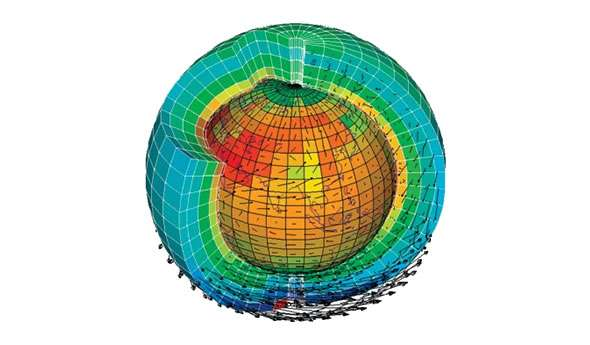
\includegraphics[scale=0.4]{maillage_terre.jpg}
	\end{center}
	\captionof{figure}{illustration d'un maillage multidimentionnel pour les modèles de climat}
	\label{fig:maillage multidimentionnel terre}
\end{figure}

La complexité des interactions entre les différents noeuds peuvent rendre les calculs vraiment laborieux. D'où l'intérêt de diminuer le nombre de mailles en en passant à grande échelle puis de downscaler les résultats obtenus. Nous présenterons dans la figure \ref{fig:modele de climat} les différentes interactions prises en compte dans l'élaboration du modèle de climat de l'IPSL.

\begin{figure}[h]
	\begin{center}
		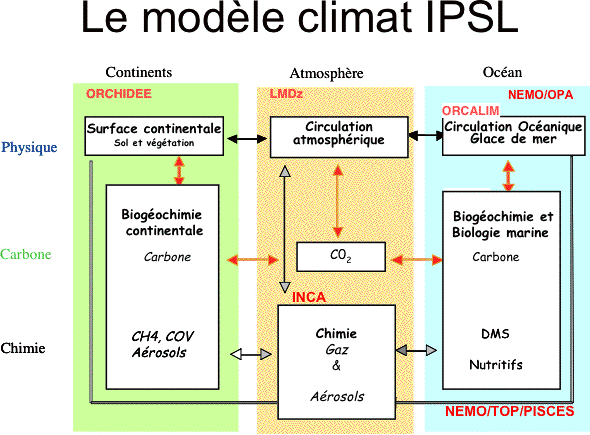
\includegraphics[scale=0.6]{modele_climat_IPSL.png}
	\end{center}
	\captionof{figure}{Présentation sommaire des différentes interactions dans le modèle de climat IPSL}
	\label{fig:modele de climat}
\end{figure}
	
Dans notre stage, nous nous sommes concentrés sur les modélisations continentales, à savoir, sur les interactions entre les modèles d'atmosphères ainsi que les mécanismes d'écoulement de l'eau dans les sols et les rivières. c'est ce que nous allons voir.

\subsection{Généralités sur les interactions atmosphère - surface continentale - sol}
\label{ch:generalite interaction atmosphere-surface continentale-sol}
Nous allons présenter ici les principales interactions entre la surface continentale et l'atmosphère, cette étude a seulement pour objectif de donner un aperçu des différentes problématiques rencontrées dans l'élaboration des modèles continentaux. En effet, nous n'avons pas eu à nous soucier de toutes ces interactions puisque les deux variables que nous avon utilisé étaient la précipitation et l'évapotranspiration potentielle, la première indiquant la quantité d'eau entrant dans le sol et la seconde la quantité d'eau sortante. Le plan de cette sous-section s'inspire très largement de la thèse \cite{maquin2016developpement}[chap 1] qui fournit d'avantage de détails et traite de la modélisation de l'ensemble des interactions dont nous allons parler. 

\subsubsection{Les écoulements}
\label{ch:ecoulement}

Les processus hydrologiques sont classiquement étudiés à l’échelle du bassin versant\footnote{Un bassin versant comme il est défini en hydrologie possède son équivalent en mathématiques, soit $(E,d)$ un espace métrique et $S:E\to E$ un endomorphisme sur $E$. On définit le bassin d'attraction d'un point $a$ qu'on appelle $B(a)$ l'ensemble des points $x$ dans $E$ tels que la suite $(x_n)_{n \in \mathbb{N}}=(S^n(x))_{n \in \mathbb{N}}$ converge vers $a$. En considérant qu'il existe une fonction $S$ définissant la trajectoire d'une goutte d'eau déposée au point $x$ les deux définitions ont la même signification en considérant le plus grand bassin d'attraction contenant un point $x$ choisi.}. En hydrologie, le bassin versant est une unité géographique définie par les limites topographiques que sont les lignes de crête. L’ensemble des écoulements converge vers les dépressions, formant ainsi un réseau hydrographique qui se dirige vers le point bas du bassin versant, l’exutoire. la figure \ref{fig:Bassin versant} définie un bassin versant. 

\begin{figure}
	\begin{center}
		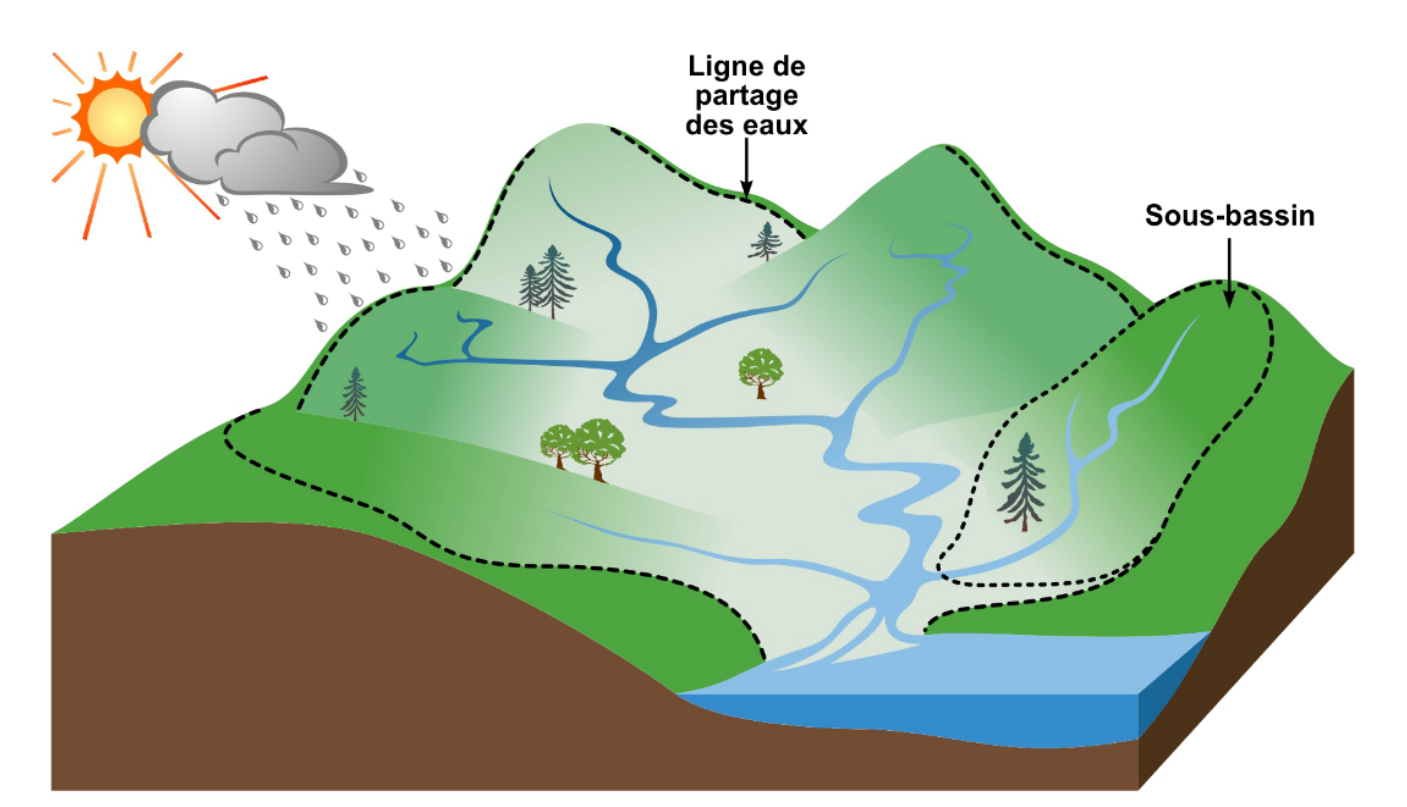
\includegraphics[scale=0.15]{bassin_versant.png}
	\end{center}
	\captionof{figure}{Bassin versant (Source :http://rqes-gries.ca/).}
	\label{fig:Bassin versant}
\end{figure}

À l’échelle du bassin versant, on distingue deux types d’écoulements: les écoulements de subsurface, les écoulements de surface. Les premiers sont des écoulements ayant lieux dans les pores du sols dans la région non saturée et les seconds en surface.


\vspace{0.7cm}

\noindent\textbf{Les écoulements de subsurface}:

La notion d'écoulement de subsurface se rapporte à l'écoulement de l'eau dans les pores du sol. Il dépend de plusieurs paramètres comme les caractéristiques du sol (sa porosité, sa perméabilité) c'est à dire la capacité qu'a l'eau à s'infiltrer dans le sol ainsi que la saturation en eau du sol, la topographie et le climat (précipitation, évaporation, transpiration). Ces écoulements sont traités par les équations de la mécanique des fluides (voir section  \ref{eq-Richards}), pour plus de détails se référer à \cite{maquin2016developpement} et \cite{marsily_de1986quantitative}. 

\vspace{0.7cm}

\noindent\textbf{Les écoulements de surface:}

Les écoulements de surface, aussi qualifiés de ruissellement apparaissent lorsque le sol est saturé en surface et que le débit d'eau sur le sol est supérieur à sa capacité d'infiltration. Deux phénomènes distincts sont responsables du ruissellement, lorsque le sol est saturé, l’eau ne peut plus s’y infiltrer \cite{cappus1960etude}. Cette condition de saturation à la surface du sol peut être la conséquence d'une nappe affleurant la surface, la zone satisfaisant cette propriété est appelée zone de suintement. Cela arrive aussi naturellement lors d'épisode pluvieux pour les nappes peu profondes. Le ruissellement peut aussi être causé par de fortes précipitations, ainsi le débit surfacique peut devenir supérieur à la quantité d'infiltration et ainsi créer un ruissellement. La quantité d'infiltration décroit exponentiellement lors d'évènements pluvieux \cite{horton1933role}.  

\begin{center}
	\captionsetup{type=figure}
	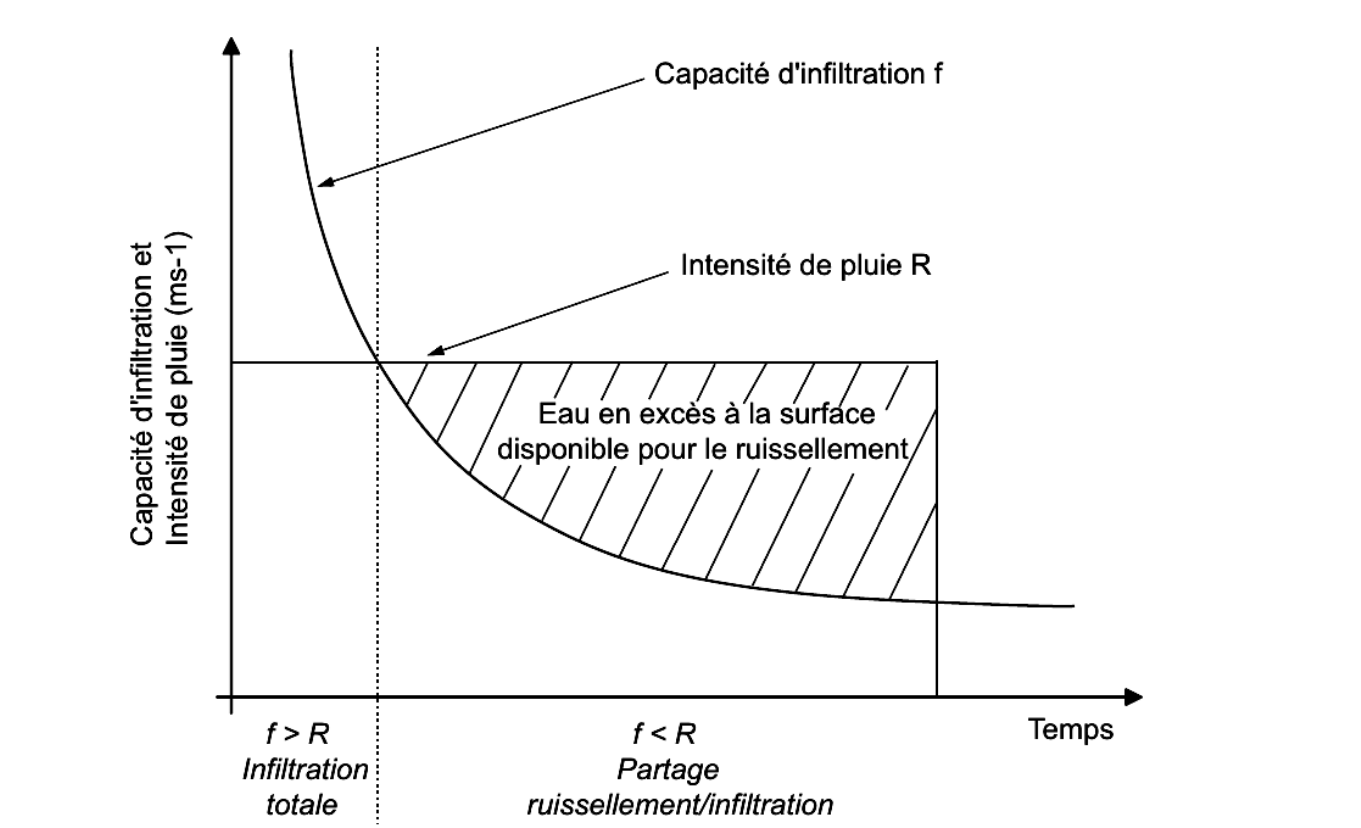
\includegraphics[scale=0.2]{ruissellement.png}
	\captionof{figure}{Estimation du ruissellement en fonction du temps, modèle de Horton(\cite{maquin2016developpement})}
\end{center} 

\vspace{0.7cm}

\noindent\textbf{Les interactions nappe rivière:}

Selon la position de la rivière par rapport à la nappe soit la nappe nourrit la rivière, soit c'est l'inverse, la figure \ref{fig:nappe_riviere} présente ce mécanisme.

\begin{figure}[h]
	\begin{center}
		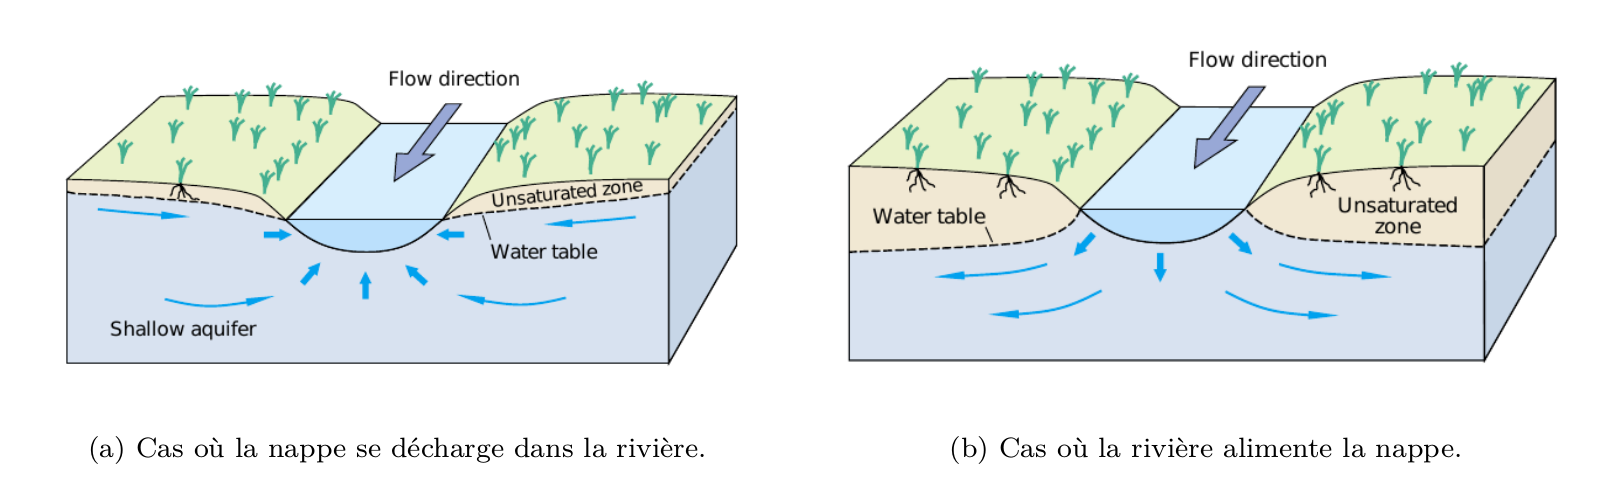
\includegraphics[scale=0.28]{nappe_riviere.png}
	\end{center}
	\captionof{figure}{Différente interactions entre la nappe et la rivière}
	\label{fig:nappe_riviere}
\end{figure}

\subsubsection{Transferts d'eau entre le sol et l'atmosphère}
\label{ch:mecanismes}

La végétation constitue le lien entre l'atmosphère et le sol. Les végétaux sont les principales voies de transfère entre le sol et l'atmosphère, via les racines et la canopée. Il y a aussi des interactions directes entre la couche de surface du sol et l'atmosphère. Les trois principaux processus décrits sont l'évaporation du sol, la transpiration des végétaux ainsi que l'évaporation de l'eau interceptée par la canopée. L'influence de la végétation a un très gros impact sur les modélisations hydrologiques, puisqu'elle influent directement sur la quantité d'eau entrant et sortant du sol. 

\vspace{0.7cm}

\noindent\textbf{la transpiration:}

La ``transpiration'' des plantes consiste en une libération de vapeur d’eau par les plantes dans l’atmosphère. Ce phénomène constitue une réponse passive à l’environnement atmosphérique dû à l’existence d’un gradient de pression positif de l’atmosphère à la canopée, on parle aussi de demande atmosphérique. L’évaporation de l’eau par les plantes se produit dans les stomates des feuilles, de petites ouvertures où s’effectuent les échanges gazeux entre l’intérieur et l’extérieur de la plante. L’ouverture des stomates peut varier, régulant ainsi le flux de transpiration. Cette variation dans l’ouverture et la fermeture des stomates dépend de différents paramètres comme l’état hydrique du végétal ou les conditions climatiques.

La transpiration amène l'eau du sol par les racines puis les stomates vers l'atmosphère, la quantité d'eau transpirée dépend aussi du volume du sol couvert par les racine ainsi que de la teneur en eau du sol. Il arrive souvent en été dans les régions arides que la densité d'eau dans le sol ne soit pas suffisante pour qu'il y ait transpiration.

\vspace{0.7cm}

\noindent\textbf{Évaporation:}

Sur les surfaces de sol non recouvertes de végétation (sol nu), l’eau présente dans le sol, à proximité de la surface, peut s’évaporer. Ce phénomène apparaît en présence d’un gradient de pression de vapeur d’eau entre le sol et l’atmosphère et d’un apport d’énergie. L’évaporation effective dépend de l’état hydrique de la surface du sol, l’énergie pour extraire l’eau du sol augmentant à mesure que le sol s’assèche et des propriétés conductrices du sol (voir \cite{hillel2003introduction}).

\vspace{0.7cm}

\noindent\textbf{Pertes par interception:}

Lors d’un épisode pluvieux, une partie de l’eau incidente est interceptée par le feuillage. Il s’agit du phénomène dit d’interception. Cette eau présente sur la canopée peut ensuite s’évaporer directement. On désigne ce processus d’évaporation sur la canopée comme les pertes par interception. L’importance de ce flux d’eau dépend de l’ampleur du feuillage et de la capacité de stockage d’eau de la canopée, c’est-à-dire de l’épaisseur maximale de la lame d’eau par unité de surface de feuillage.

\vspace{0.7cm}

\noindent\textbf{l'évapotranspiration potentielle:}

On désigne par  ``évapotranspiration potentielle'' la quantité d’eau maximale que l’atmosphère peut extraire via les trois processus décrits précédemment. Elle correspond ainsi à la demande atmosphérique évoquée auparavant. Elle correspond à la quantité d'eau fournie par un sol saturé en eau. Les articles \cite{kristensen1975model}, \cite{zhifang2010estimation} donnent des méthodes pour passer de l'évapotranspiration potentielle à l'évapotranspiration réelle, cependant il semble que ce sujet soit encore controversé dans la communauté des hydrologues.  

\subsection{Les concepts hydrologiques: modélisation de l'écoulement dans le sol}
\label{hydro}

Nous allons ici introduire les principales notions propres à l'étude hydrologique des sols. Plusieurs caractéristiques définissent un sol, mais avant d'étudier  plus en détail ce qui définit un sol, il est important de comprendre que l'étude hydrologique d'un sol est simplement un bilan d'eau dans celui-ci. De facon plus générale, la grandeure qui va nous intéresser dans notre étude ne sera pas la hauteur de nappe, mais les débit de l'eau sortante.
Il faut alors commencer par déterminer ce qui rentre et ce qui sort. L'estimation de ces quantités est l'objet d'étude du downscaling qui cherche à prévoir la précipitation et l'évapotranspiration potentielle.

\subsubsection{Quelques définitions pour l'étude en milieu poreux}
\label{ch: definition milieu poreux}
On comprends intuitivement que la nature du sol aura un impacte dans l'écoulement de l'eau. par exemple un sol très sableux permet un écoulement beaucoup plus rapide qu'un sol argileux. Ceci est lié au volume de vides relatifs. Nous introduirons ici les concepts principaux de l'étude hydrologique en milieu poreux.

\begin{definition}
	On appelle \textbf{porosité totale $\omega$} la valeur définie par
	\begin{equation}
		\omega =\frac{\textrm{Volume des vides}}{\textrm{Volume total de la roche}}.
	\end{equation}
	On appelle aussi \textbf{indice des vides $e$} la valeur définie par 
	\begin{equation}
		e=\frac{\textrm{Volume des vides}}{\textrm{Volume du solide plein}}.
	\end{equation}
	On peut passe d'une formule à l'autre par la relation 
	\[e\omega=e-\omega.\]
\end{definition}
L'on peut trouver des méthodes de mesure de la porosité d'un sol dans l'ouvrage (\cite{marsily_de1986quantitative}). On dit aussi que le sol n'est pas saturé lorsque l'eau n'a pas pris tout l'espace disponible, on parle alors de saturation volumique. Ce concept est fondamental pour comprendre la dynamique de l'écoulement, par exemple en dessous d'une certaine saturation les forces de capillarités seront plus fortes que celles de gravité et il n'y aura aucun écoulement.
 
\begin{definition}
	On parle de \textbf{saturation volumique $\theta$}, la saturation définie par le rapport
	\begin{equation}
		\theta= \frac{\textrm{Volume d'eau contenu}}{\textrm{Volume total}},
	\end{equation}
	on a $0\leq<\theta\leq \omega$. Et la \textbf{saturation volumique $s$}
	\begin{equation}
		s=\frac{\textrm{Volume d'eau contenu}}{\textrm{Volume total des pores}}.
	\end{equation}
\end{definition}

En fonction de la saturation volumique les échelles de temps et les forces misent en action ne sont pas les mêmes.


\subsubsection{Les équations pour modéliser l'écoulement}
\label{ch: eq meca-flu}
L'objet de cette section sera de montrer quelques équations fondamentales que manipulent les hydrologues pour modéliser les écoulements en milieu poreux. Nous allons par la suite montrer la démarche physique permettant d'obtenir ces équations. On commence par rappeler les équations de la dynamiques des fluides. L'équation de de conservation de la matière:
\begin{equation}
	\label{cons-mat}
	div(\rho \overrightarrow{u})+\frac{\partial \rho}{\partial t}=0.
\end{equation}
Où $\rho$ est la masse volumique et $\overrightarrow{u}$ le vecteur vitesse du fluide. On écrit maintenant l'équation de Navier-Stokes
\begin{equation}
	\frac{\partial p}{\partial x^i}-(\zeta+\frac{\mu}{3})\frac{\partial}{\partial x^i}(div\overrightarrow{u}) - \mu \nabla^2u^i=\rho(F^i -\frac{du^i}{dt}).
\end{equation}
$\zeta$ coefficient de viscosité du volume, (très souvent négligeable devant $\mu$) $[ML^{-1}T^{-1}]$,\\
$\mu$ coefficient de viscosité dynamique, $[ML^{-1}T^{-1}]$\\
$\nabla^2$ le laplacien,\\
$F^i$ composante des forces à distance par unité de masse,\\
$i$ un vecteur unitaire de l'espace $3D$.

En milieu poreux les équations de Navier-Stokes deviennent difficilement applicables car le milieu dans lequel s'écoule le fluide dépend lui-même de l'écoulement du fluide. On peut en effet imaginer que la porosité augmente avec la vitesse d'écoulement (si on considère la géométrie uniforme et la porosité). On va alors simplifier l'équation de Navier-Stokes en posant certaines hypothèses propres au milieu dans lequel on les étudie. 

\vspace{0.7cm}

\noindent \textbf{Hypothèses simplificatrices:}\\
En milieu poreux on peut émettre de nombreuses hypothèses simplificatrices qui permettent de simplifier l'équation de Navier Stokes, on peut supposer les écoulement permanents
\[\frac{\partial u^i}{\partial t}=0,\]
on suppose aussi que le fluide est incompressible ($\rho$ constant) alors
\[div(\rho \overrightarrow{u})=-\frac{\partial \rho}{\partial t}=0,\]
et finalement,
\[div \overrightarrow{u}=0.\]
Dans ces hypothèses l'équation de Navier-Stokes devient
\begin{equation}
	\label{eq-cons-m-simp}
	\frac{\partial p}{\partial x^i}-\mu \nabla^2u^i-\rho F^i=0. 
\end{equation}

Plusieurs méthodes numériques permettent de trouver des solutions à ce problèmes notamment la méthode de Galerkine ou des méthodes de différences finies voir \cite{allaire2005analyse} (chap 2, chap 6). 

\vspace{7mm}

Remarquons que ces équations ne prennent pas en compte la porosité du milieu, l'équation \eqref{cons-mat} peut être modifié en prenant en compte $\omega$ le coefficient de porosité et un terme source $q$ lié à la matière créant des interstices sans fluide (le coefficient est compté négativement). Alors l'équation de conservation devient en milieu poreux.
\begin{equation}
	\label{eq:mass-por}
	div(\overrightarrow{U})+\frac{\partial}{\partial t}(\theta)+ q=0.
\end{equation}
Remarquons que l'on considère la porosité $w$ comme continue nous étudions des éléments de longueures $dx$ suffisamment petite pour que les équations de continuité \eqref{eq-cons-m-simp} et \eqref{eq:mass-por} soient considérée vrais et suffisamment grandes pour que l'on puisse considérer une porosité moyenne dans un élément de volume.

\subsubsection{La loi de Darcy et l'équation de diffusivité en milieu poreux}
\label{Darcy}
Henry Darcy, alors qu'il étudiait les fontaines de la ville de Dijon (1856) établit expérimentalement que le débit d'eau s'écoulant à travers un massif de sable peut se calculer.

\begin{figure}[!h]
	\begin{center}
		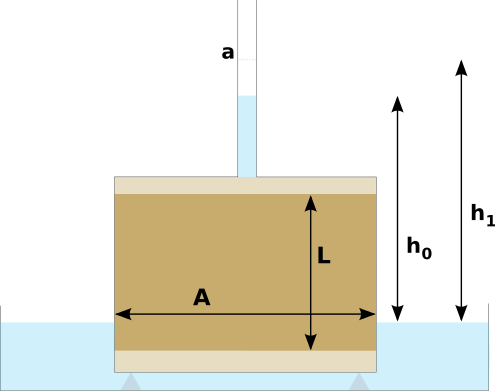
\includegraphics[scale=0.4]{darcy.png}
		\captionof{figure}{Schéma de l'équipement utilisé par Darcy pour obtenir l'équation \eqref{eq-Darcy}}
	\end{center}
	\label{fig:Darcy}
\end{figure}

Il en déduisit une formule expérimentale
\begin{equation}
	\label{eq:Darcy}
	Q=KA\frac{\Delta h}{L}.
\end{equation}
$Q$ est le débit volumique s'écoulant à travers  
$A$ est la section du massif sableux\\
$\Delta h$ la perte de charge\footnote{En hydraulique la charge est une grandeur homogène à une longueur, on l'exprime parfois sous la forme d'une pression: $cste\times\rho g$. Sinon on pose souvent \[h=\]} de l'eau entre le sommet et la base du massif sableux\\
$K$ est une constante dépendant du milieu poreux, baptisée coefficient de perméabilité\\
$L$ est l'épaisseur du massif sableux.



\vspace{0.7cm}

On appelle $U=Q/A$ \textbf{la vitesse de filtration} d'un sol. À partir des équations de Navier-Stokes on sait que les causes du déplacement du fluide sont dûs au gradient de pression ainsi qu'aux forces extérieures. La loi de Darcy peut alors s'exprimer sous la forme générale
\begin{equation}
	\label{eq-Darcy}
	\overrightarrow{U}=\frac{k}{\mu }(\overrightarrow{\nabla}\, p+\rho g \,\overrightarrow{\nabla}\, z).
\end{equation} 

On peut réécrire cette équation
\[\overrightarrow{U}=-K(\overrightarrow{\nabla}\, h + \,\overrightarrow{\nabla}\, z),\]
avec $K=k(\mu \rho g)^{-1}$ $[LT^{-1}]$ et $h=p(\rho g)^{-1}$ $[L]$. En posant 
\[H=h+z,\]
on peut alors injecter l'équation de Darcy \eqref{eq-Darcy} dans l'équation de conservation de la masse \eqref{eq:mass-por} pour finalement obtenir
\begin{equation}
	\label{eq-Richards}
 	-\overrightarrow{\nabla} \cdot (K\overrightarrow{\nabla}H)+\frac{\partial\theta}{\partial t}+ q=0.
\end{equation}  
On définit parfois des lois de porosité liées à la grandeur $f(H)=\theta$ la quantité d'eau est liée à la cote piézométrique \footnote{Le niveau, la cote ou la surface piézométrique est l'altitude ou la profondeur (par rapport à la surface du sol) de la limite entre la nappe phréatique et la zone vadose dans une formation aquifère. Ce niveau est mesuré à l'aide d'un piézomètre.} et l'on pose 
\[S_s(H)\frac{\partial H}{\partial t}=\frac{\partial\theta}{\partial t},\]
$S_s$ est appelé le coefficient d'emmagasinement. On appelle l'équation ainsi obtenu en injectant la formule sur la porosité, \textbf{l'équation de Richard généralisée}
\begin{equation}
	\label{eq-ge-richard}
	S_s(H)\frac{\partial H}{\partial t}-\overrightarrow{\nabla} \cdot (K(\theta)\overrightarrow{\nabla}H)+q=0.
\end{equation}

Ceux sont avec ces équations que les hydrologues travaillent. Nous pouvons remarquer que cette simplification des équations peut être considérée comme le début d'un processus d'upscaling. On cherche à simplifier le modèle pour qu'il soit encore vrai à grand échelle. Notons que les équations de Darcy ont été justifiées dans les travaux de Matheron et Marle à partir de l'intégration dans un milieu réel des équations de Navier. 

\subsection{Les modèles hydrologiques et la problématique de l'upscaling}
\label{ch:modeles-hydro-upscaling}
Nous allons présenter dans cette partie deux modèles hydrologiques, le premier HydroGéoSphère est celui que nous avons utilisé pour réaliser les modélisations hydrologiques sur le bassin du Little Washita, le second Orchidée est le modèle de surface continentale utilisé par l'IPSL. 

\subsubsection{Le modèle d'hydrogéosphère}

HydroGéoSphère (HGS) est un code de calcul hydrologique tri-dimensionnel, intégré et à base physique. Il a été développé par R. Therrien puis conjointement à l’Université de Laval, à Québec et à l’Université de Waterloo. Ce code de calculs permet de simuler les écoulements de surface et de subsurface, ainsi que le transport de solutés et d’énergie de manière intégrée, c’est-à-dire que les équations gouvernant ces processus sont résolues simultanément. Le code est parallélisé permettant une efficacité numérique élevée et donc des applications à des échelles spatio-temporelles importantes.

À chaque pas de temps le modèle résout les équations de transport d'eau de surface et de subsurface ainsi que celles conservation de la masse en même temps. En regardant la figure \ref{fig:HGS_water_balance} on a la conservation des quantités d'eau en surface s'écrit
\begin{equation}
	\label{eq:HGS-surface}
	P = (Q_{S2}-Q_{S1})-Q_{GS}+I+ET_S+Q^W_S+\Delta S_S /\Delta t,
\end{equation}
et les équations de subsurface s'écrivent
\begin{equation}
	\label{eq:HGS-subsurface}
	I = (Q_{G2}-Q_{G1})+Q_{GS}+ET_G + Q^W_G+\Delta S_G/\Delta t.
\end{equation}
On a finalement,
\begin{equation}
	\label{eq:HGS-bilan-tot}
	P=(Q_{S2}-Q_{S1})+(Q_{G2}-Q_G1)+(ET_S+ET_G)+(Q^W_S+Q_G)+(\Delta S+S+\Delta S_G)/\Delta t
\end{equation}
Avec $Q_{S1}$ et $Q_{S2}$ les flux entrant et sortant, $Q_{GS}$ le flot d'interaction entre la surface et la subsurface, $ET_S$ l'évapotranspiration de surface. $Q^W_S$ et $Q^W_G$ les termes puits définis précédemment \eqref{eq:mass-por}. $\Delta S_S$ et $\Delta S_G$ les différences de stockage d'eau en surface et en subsurface sur le temps $\Delta t$.

\begin{figure}[h]
	\begin{center}
		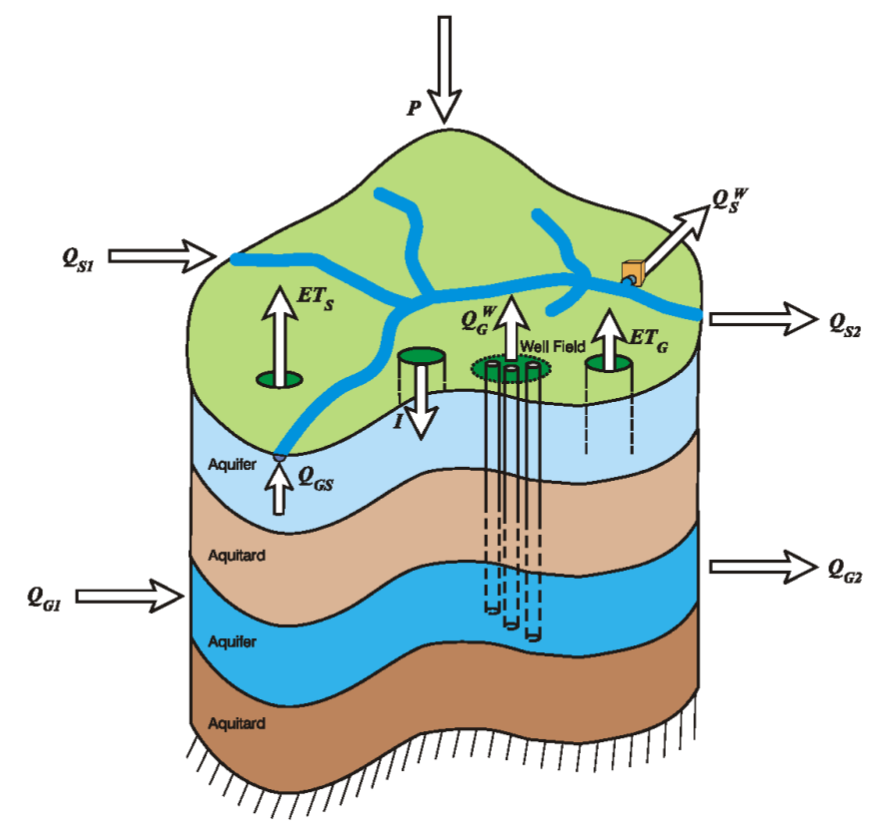
\includegraphics[scale=0.35]{HGS_modele.png}
	\end{center}
	\captionof{figure}{Schéma des cycles hydrologiques pris en compte par hydrogéosphère}
	\label{fig:HGS_water_balance}
\end{figure}

Hydrogésphère résout rigoureusement les équations de la physiques cités dans la partie \ref{ch: eq meca-flu} et donne des résultats très précis. Cependant la capacité informatique actuelle ne permet pas d'implémenter HydroGéoSphère dans un modèle de climat. Il fallait créer des modèles plus simples et plus grossiers pour résoudre le problème à plus grande échelle. C'est le principe du modèle continentale Orchidée. 

\subsubsection{Le modèle d'Orchidée}

Orchidée est un modèle continentale dans le continuum sol-végétation-atmosphère. Ses résultats sont intégrés comme condition à la limite basse du modèle générale de circulation atmosphérique du Laboratoire de Météorologie Dynamique. Orchidée simule en particulier les flux d’énergie, d’eau et de carbone entre les surfaces continentales et l’atmosphère. Il est composé de trois modules qui représentent des processus différents et agissant à des échelles de temps différentes: SECHIBA (Schématisation des Échanges Hydriques à l’Interface entre la Biosphère et Atmosphère), STOMATE, qui modélise principalement la phénologie végétale (les phases de développement saisonnier des plantes liées au cycle climatique annuel et les échanges de carbone dans la biosphère, et LPJ qui simule l’évolution dynamique de la végétation. Dans le cadre de ce stage, seul le module SECHIBA a été étudié.

La description que nous allons en donner ici est très sommaire et rassemble ce que nous en avons compris de la discussion que nous avons eu avec Emmanuel Mouche et de la lecture de la présentation \cite{gumiberteau2016}. Le modèle d'Orchidée est un modèle de réservoir, c'est à dire qu'on discrétise l'espace en plusieurs zones qui peuvent contenir de l'eau. Nous avons vu qu'il y avait plusieurs types d'écoulements qui intervenaient à différentes échelles de temps et à différents endroits dans le sol. Orchidée considère alors trois types de transfère d'eau dans trois types de réservoirs. Les écoulements considérés sont: les écoulements de surface, de subsurface et finalement les échanges entre la rivière et la nappe. 

\begin{figure}[h]
	\label{fig:HGS}
	\begin{center}
		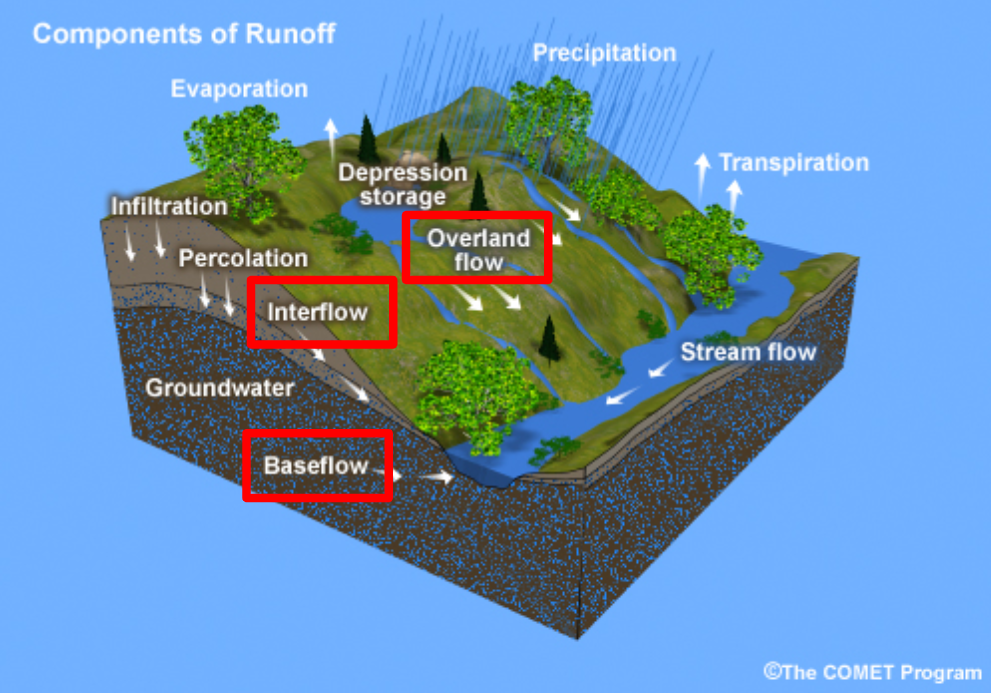
\includegraphics[scale=0.3]{different_flows.png}
	\end{center}
	\captionof{figure}{Schéma des cycles hydrologiques pris en compte par Orchidée}
\end{figure}

Alors dans chaque block considérer il y a trois réservoirs d'eau. Un réservoir pour les écoulements écoulements de surface, un pour les écoulements de subsurface et un pour les interaction nappe-rivière. La figure \ref{fig:Orchidee-interact} présente les différente intéractions entre deux blocks.


\begin{figure}[h]
	\begin{center}
		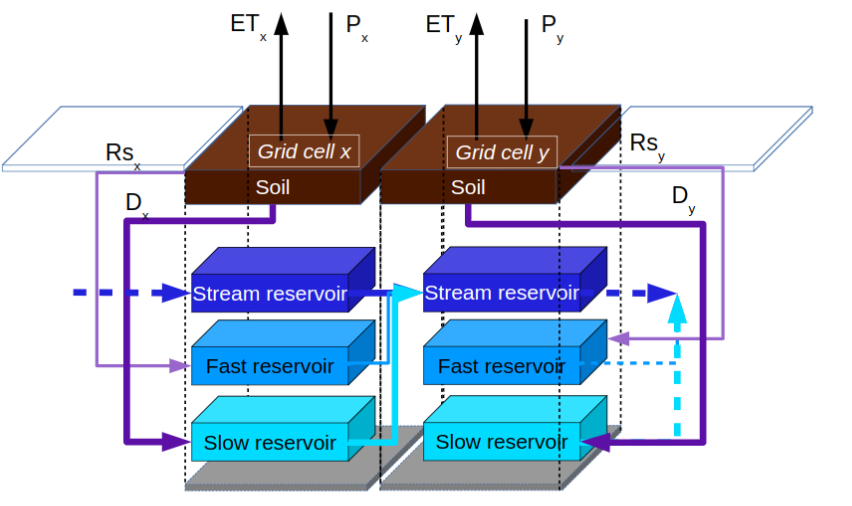
\includegraphics[scale=0.3]{Orchidee_interaction.png}
		
	\end{center}
	\captionof{figure}{Modèle de réservoir utilisé par Orchidée, image issue de \cite{gumiberteau2017}}
	\label{fig:Orchidee-interact}
\end{figure}

Remarquons que la couche du haut, dont nous n'avons pas parlé est le sol sur lequel on considère les précipitations ($P_X$, $P_Y$) et l'évapotranspiration ($ET_X$,$ET_Y$). Le \textit{stream reservoir} est le réservoir des écoulements de surface, le \textit{fast reservoir} correspond au réservoir des écoulements de subsurfaces et le \textit{slow reservoir} correspond à la nappe. Les écoulements verticaux $(Rs_X,Rs_Y)$ et $(D_X,D_Y$) simulent les proportions des précipitations stocké dans chaque sous-block, et le calcule de $Rs$ et $D$ en fonction des précipitations est détaillé dans la présentation \cite{gumiberteau2017}. On peut remarquer que d'après ce schéma il n'y a pas d'écoulement de surface.
On peut remarquer ensuite que les écoulement vont seulement d'un réservoir à l'autre, ce paradigme semble raisonnable puisque les écoulements vont eux toujours dans le sens de la pente. Un autre partie pris est qu'un block ne se déverse que dans un seul et unique block, ce comportement semble légitime si l'on considère qu'il n'arrive que très rarement qu'une rivière se divise dans le sens de l'aval. Néanmoins, considérant la surface des blocks ($>0.5^{\circ}$), il est fréquent que plusieurs bassins soient contenus dans le même block et alors ce choix devient discutable.

\subsubsection{Conclusion et étude des modèles}

Ayant vu deux modélisations d'une surface continentale, leur comparaison peut enrichir la réflexion de l'upscaling. 

-Propriétés intéressantes: Convergence d'un modèle à l'autre en faisant tendre la longeure de maille vers 0?

-Comment mesurer la distance? Segmenter le modèle d'HydroGéoSphère en trois réservoire et regarder les bilans sur les différents réservoirs.

-Commencer par résoudre les équations de la physique dans chaque réservoir?

-Quantifier la différence au modèle réel.

Cette étude pourrait faire l'objet d'un stage ou d'une thèse entière. 


\newpage
\section{Projections Climatiques et modélisation hydrologique}
\label{ch:Proj-climatique-mod-hydro}

Dans cette section nous présentons les résultats que nous avons obtenus par l'analyse des données NARR sur le bassin du Little Washita. L'organisation de notre travail est résumé dans la figure \ref{fig:methodo}.

Commençons par rappeler les enjeux de ce stage. Nous cherchons à étudier l'impact du changement d'échelle sur les prédictions climatiques et les modélisations Hydrologiques. Avant de commencer notre travail, nous avons commencé par faire une étude de la région du Little Washita ainsi que des données NARR. Pour étudier la problématique du changement d'échelle nous avons voulu étudier l'impact de différents changements d'échelles. Nous avons donc considéré des dégradations des données NARR sur plusieurs échelles (le processus de dégradations est expliqué dans la section \ref{ch:degradation}). On commence par considérer les variables de précipitation et d'évapotranspiration sur un point de maille NARR (le point couvrant la majeur partie du bassin du Little Washita) donc de $32km\times 32km$ puis nous avons considéré la moyenne des précipitations sur des ensembles de mailles entourant le point correspondant au Little Washita sur des surfaces de plus en plus grandes (voir section \ref{ch:degradation}). Finalement nous avons considéré le jeux de données du modèle de climat de l'IPSL qui possède une largeur de maille supérieur ($200km\times 200km$). Une fois récupérer les séries des réalisations des variables à ces différentes échelles nous avons appliqué la méthode CDF-t pour downscaler ces séries et donc transformé les données à grande échelle pour améliorer les projections sur la maille du Little Washita. Nous avons ensuite simulé la modélisation hydrologique pour toutes nos séries de précipitation et d'évapotranspiration. Finalement, nous avons étudiés et comparer les résultats des débits renvoyés par les différentes simulations. Mais comme un schéma vaut mieux qu'un long discours voici un schéma résumant notre travail sur les données NARR.

\begin{figure}[h]
	\begin{center}
		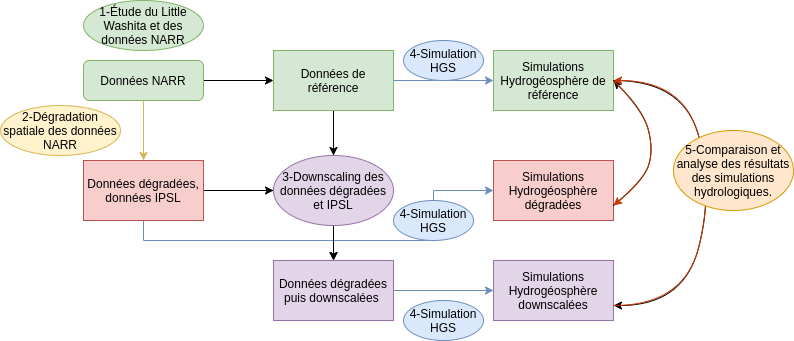
\includegraphics[scale=0.6]{Diagrame_methodo.png}
	\end{center}
	\captionof{figure}{Plan d'étude du stage}
	\label{fig:methodo}
\end{figure}

\subsection{Analyse des données NARR}


















\newpage
\section{Annexes}

\subsection{Annexe: Preuves et outils utilisés dans le downscaling}
\label{ch:outils-mathematiques}
\begin{proposition}
	Soit $X$ et $Y$ deux variables aléatoires réelles ayant des fonctions de répartition $\mathcal{F}_{X}$ et $\mathcal{F}_{Y}$ continues, alors 
	$\mathcal{F}^{-1}_Y (\mathcal{F}_X(X))$ et $Y$ suivent la même loi. 
\end{proposition}
\begin{proof}
	Montrons que $\mathcal{F}^{-1}_Y \circ \mathcal{F}_X(X)$ et $Y$ possède la même fonction de densité. 
	\[\mathcal{F}_{\mathcal{F}^{-1}_Y \circ \mathcal{F}_X(X)}(y)
	= \mathbb{P}(\mathcal{F}^{-1}_Y (\mathcal{F}_X(X))\leq y )
	= \mathbb{P}(\mathcal{F}_{X}(X) \leq \mathcal{F}_Y(y)),\]
	comme $\mathcal{F}_{X}(X)$ suit une loi uniforme sur $[0,1]$ si $F_X$ est continue cette égalité se réécrit
	\[= \mathbb{P}(\mathcal{U}(0,1) \leq \mathcal{F}_Y(y))=\mathcal{F}_Y(y).\]
\end{proof}
\begin{proposition}
	\label{mean-rep-emp}
	Soient $X_1,...,X_n$ n réalisations d'une variable aléatoire réelle $X$ et $\mathcal{F}_{n}$ sa fonction de répartition empirique nous avons
	\[E[\mathcal{F}_n]=F_{X},\]
	alors la fonction de répartition empirique est un estimateur sans biais de la lois de $F$. 
\end{proposition}

\begin{proof}
	C'est en effet évident puisque $\mathds{1}_{[X, +\infty )}(x)$ suit une lois de Bernoulli de paramètre $\mathcal{F}(x)$ alors 
	\[E\Big[\frac{1}{n}\sum_{i=1}^{n}\mathds{1}_{[X_i, +\infty )}(x)\Big]= \frac{1}{n}\sum_{i=1}^{n}E[\mathds{1}_{[X_i, +\infty )}]=\mathcal{F}_{X}(x).\]
\end{proof}


\begin{theorem}(Glivenko-Cantelli)
	\label{th:glivenko}
	Soient $\mathcal{F}_{X}$ et $\mathcal{F}_{n}$ respectivement la fonction de répartition et la fonction de répartition empirique. Alors 
	\begin{equation}
		\|\mathcal{F}_{X}-\mathcal{F}_{n}\|_{\infty} \xrightarrow[n\to \infty]{prob} 0.
	\end{equation}
\end{theorem}

\begin{proof} (Cas où $\mathcal{F}_X$ est continue)
	On commence par remarquer que quelque soit $x$ dans $\mathbb{R}$, \[F_{n}(x)\xrightarrow[n\to \infty]{p.s.}\mathcal{F}_X(x)\] d'après la loi forte des grands nombres et la proposition \eqref{mean-rep-emp}. Pour q dans $\mathbb{Q}$, on définit 
	\[\Omega_{q}=\{\omega \in \Omega | \lim_{n \to \infty} \mathcal{F}_{n}(q)=\mathcal{F}_X(q)\},\]
	d'après ce que nous avons dit, sa mesure pour la probabilité $P(\Omega_q)=1$ comme $\mathbb{Q}$ est dénombrable nous avons  
	\[P\Big(\bigcap_{q \in \mathbb{Q}} \Omega_q \Big)=1.\]
	Alors, comme $\mathbb{Q}$ est dense dans $\mathbb{R}$ et que $\mathcal{F}_{X}$ et les $(\mathcal{F}_n)_{n \in \mathbb{N}}$ sont continues on peut assurer que   
	\[	\|\mathcal{F}_{X}-\mathcal{F}_{n}\|_{\infty} \xrightarrow[n\to \infty]{prob} 0. \]
\end{proof}
Le cas où $\mathcal{F}_{X}$ n'est pas continue est géré par \cite{durrett2019probability} (ex 7.2 chap 1). On voit d'après le théorème \ref{th:glivenko} que la fonction de répartition empirique est le bon estimateur de la fonction de répartition. 


\subsection{Annexe: La statistique de Cramér-von Mises}
\label{lemme Cramer-von Mise}
Soient $(X_i)_{i\in \llbracket 1,n \rrbracket}$ et $(Y_i)_{i\in \llbracket 1,m \rrbracket }$ des réalisations indépendante issues des variables aléatoires réelles $X$ et $Y$. On appelle $\mathcal{F}_{n}$ et $\mathcal{G}_{m}$ les fonctions de répartitions empiriques définies à partir de ces réalisation et $\mathcal{H}_{m,n}$ la fonction de répartition empirique définie à partir des réalisations $(Z_i)_{i\in \llbracket 1,m+n \rrbracket }=X_1,...,X_n,Y_1,...,Y_m$. Par la suite on considéra que tous les éléments sont triés dans leur ensemble (c.à.d. $i\leq j \Rightarrow E_i\leq E_j$). Nous avons alors l'égalité suivante
\begin{equation}
	C_{n,m}=\frac{nm}{n+m}\int_{\mathbb{R}}\big[ \mathcal{F}_{n}(x)-\mathcal{G}_{m}(x)\big]^{2} \mathrm{d} \mathcal{H}_{m,n}(x)=\frac{1}{nm(m+n)}\Big[ n\sum_{i=1}^{n}(R_{X_i}-i)^2+ m\sum_{i=1}^{m}(R_{Y_i}-i)^2\Big]-\frac{4nm-1}{6(m+n)}.
\end{equation}
où $R_{Z_i}$ est le rang de $Z_i$ dans $X_1,...,X_n,Y_1,...,Y_n$ autrement dit 
\[R_{X_i}=Card(\{j \in \llbracket 1,m+n \rrbracket , Z_j\leq Z_i\}).\] 
Notons que cette égalité transforme un problème d'analyse en un problème de dénombrement beaucoup plus simple. On rappelle la définition de l'intégrale par rapport à une fonction.
\begin{definition}
	Soient $f:\mathbb{R} \to \mathbb{R}$ et $g:\mathbb{R} \to \mathbb{R}$ deux fonctions continues par morceaux on définit l'intégrale de $f$ par rapport à $g$ comme étant
	\[\int_{\mathbb{R}}f(x)\, dg(x)=lim_{n\to\infty}\sum_{i \in \mathbb{Z}}f(x_{i,n})\big( g\big(x_{i,n}\big)-g\big(x_{i,n-1})\big),\hspace{4mm}x_{i,n}=i/n.\]
\end{definition}

\begin{proof}
	
	\noindent Commencons par montrer l'égalité
	\[\frac{nm}{n+m}\int_{\mathbb{R}}\big[ \mathcal{F}_{n}(x)-\mathcal{G}_{m}(x)\big]^{2} \mathrm{d} \mathcal{H}_{m,n}(x)=\frac{mn}{(m+n)^2}\sum_{i=1}^{m+n}\big(\mathcal{F}_n(Z_i)-\mathcal{G}_{m}(Z_i)\big)^2.\]
	On pose $\delta=\inf \{|Z_i-Z_j|, Z_i \neq Z_j\}$, quel que soit $n\geq n_0$ tel que $1/n_0< \delta$ on a: 
	\[\sum_{i \in \mathbb{Z}}\big(\mathcal{F}_n(\frac{i}{n})-\mathcal{G}_{m}(\frac{i}{n})\big)^2\Big( \mathcal{H}_{m,n}\big(\frac{i}{n}\big)-\mathcal{H}_{m,n}\big(\frac{i-1}{n}\big)\Big)=\sum_{i=1}^{m+n}\big(\mathcal{F}_n(Z_i)-\mathcal{G}_{m}(Z_i)\big)^2,\]
	on obtient donc directement l'égalité voulue en passant à la limite.
	
	Observons maintenant que $\mathcal{F}_n(X_i)=i/n$ et $\mathcal{G}_m(X_i)=(R_{X_i}-i)/m$ ainsi que $\mathcal{F}_n(Y_i)=(R_{Y_i}-i)/n$ et $\mathcal{G}_m(X_i)=i/m$. On peut alors réécrire $C_{n,m}$ en séparant la somme sur les $X_i$ et $Y_i$
	\[C_{n,m} = \frac{mn}{(m+n)^2}\Big[\sum_{i=1}^{n} \Big(\frac{i}{n}-\frac{R_{X_i}-i}{m}\Big)^2+ \sum_{i=1}^{m}\Big(\frac{R_{Y_i}-i}{n}-\frac{i}{m}\Big)^2 \Big]\]
	\[=\frac{mn}{(m+n)^2}\Big[\frac{1}{m^2}\sum_{i=1}^{n}\Big(R_{X_i}-i\frac{m+n}{n}\Big)^2 +
	\frac{1}{n^2}\sum_{i=1}^{m}\Big(R_{Y_i}-i\frac{m+n}{m}\Big)^2\Big]\]
	Remarquons que $C_{n,m}$ est de la forme
	\[C_{n,m}=\frac{mn}{(m+n)^2}\Big[\frac{C_1}{m^2}+\frac{C_2}{n^2} \Big],\]
	et que $C_1$ et $C_2$ sont symétriques en $n$ et $m$. On définit $\Sigma_1=\sum_{i=1}^{n}R^{2}_{X_i}$, $\Sigma_2=\sum_{i=1}^{m}R^{2}_{Y_i}$ et $\mathcal{S}_{k}=\sum_{i=1}^{k}i^2$ nous allons travailler sur l'expression
	\[C_1=\sum_{i=1}^{n}\Big(R_{X_i}-i\frac{m+n}{n}\Big)^2.\]
	On la développe puis factorise pour obtenir
	\[C_1=\frac{m+n}{n}\sum_{i=1}^{n}(R_{X_i}-i)^2-\frac{m}{n}\Sigma_1+\frac{m(m+n)}{n^2}\mathcal{S}_n.\]
	On obtient de la même manière
	\[C_2=\frac{m+n}{m}\sum_{i=1}^{m}(R_{Y_i}-i)^2-\frac{n}{m}\Sigma_2+\frac{n(m+n)}{m^2}\mathcal{S}_m.\]
	D'après ce qu'on a dit précédemment on a donc: 
	\[C_{n,m}=\frac{1}{nm(m+n)}\Big[ n\sum_{i=1}^{n}(R_{X_i}-i)^2+ m\sum_{i=1}^{m}(R_{Y_i}-i)^2\Big]-\frac{\Sigma_1+\Sigma_2}{(m+n)^2}+ \frac{\mathcal{S}_n}{n(n+m)}+ \frac{\mathcal{S}_m}{m(m+n)}.\]
	
	On remarque $\Sigma_1+\Sigma_2 = \mathcal{S}_{m+n}$ et que l'on a la première moitié de notre somme. 
	Il ne reste plus qu'à développer l'expression 
	\[-\frac{\mathcal{S}_{m+n}}{(m+n)^2}+ \frac{\mathcal{S}_n}{n(n+m)}+ \frac{\mathcal{S}_m}{m(m+n)}\]
	\[=-\frac{(m+n+1)(2m+2n+1)}{6(m+n)}+ \frac{(n+1)(2n+1)}{6(m+n)}+\frac{(m+1)(2m+1)}{6(m+n)}=-\frac{4mn-1}{6(m+n)}\]
	En regroupant nos deux résultats nous avons finalement:
	\[C_{n,m}=\frac{1}{nm(m+n)}\Big[ n\sum_{i=1}^{n}(R_{X_i}-i)^2+ m\sum_{i=1}^{m}(R_{Y_i}-i)^2\Big]-\frac{4nm-1}{6(m+n)}\]
\end{proof}	


\newpage
\bibliographystyle{apalike} 
\bibliography{mabib}

\end{document}